\renewcommand\categorylabel{[PROJEKT.EINBLICK]}

\renewcommand\authorsline{Vorname Nachname, Vorname Nachname, Vorname Nachname, ...}

\stylesectionMC{Mensch-Maschine-Interaktion im virtuellen Raum erproben: Der Fahrsimulator des KIT-IFAB\label{sec:ifab}}{Die Interaktion zwischen Mensch und Fahrzeug spielt eine zentrale Rolle -- in Bezug auf Sicherheit, Komfort und Effizienz. Das hat auch der technische Fortschritt durch neue Mobilitätslösungen nicht geändert, im Gegenteil: Durch Automatisierung und neue Interaktionskonzepte ist das Zusammenspiel wesentlich komplexer geworden. Um Assistenzsysteme und automatisierte Fahrfunktionen zu entwickeln, in denen die Insassen mitgedacht sind, Institut für Arbeitswissenschaft und Betriebsorganisation (IFAB) am KIT einen Fahrsimulator, der umfangreiche Probandenstudien ermöglicht. Wir werfen einen Blick vor Ort auf die Technik und die damit verbundenen Möglichkeiten.
\vspace{-10pt}% <- Das vspace ist für das konkrete Layout mit dem Hintergrundbild nötig, das kann je nachdem auch entfallen.
}
{% Was in diesen Klammern steht, wird am Anfang der Seite ausgeführt. Wenn ihr alles hier drin auskommentiert erhaltet ihr einen "normalen" Beitrags-Anfang.
\vspace{5.5cm} % Verschieben der Überschrift
\replaceSSColor{white}% Wenn man diese Zeile auskommentiert, sind die Titeltexte dunkelblau und grün (ihre Normalwerte), für den schwarzen Hintergrund werden sie hier in diesem Beitrag auf weiß gesetzt.
\ThisULCornerWallPaper{1.007}{content/caudri/images/ifab1c}% Hintergrundbild
\pagecolor{black} % Farbseite
}




\afterpage{%
\resetSSColor
}


% Dieser Block {\mediumfamily\color{white}...} ist nötig weil der Hintergrund der ersten Seite im IFAB-Beitrag schwarz ist. Ihr könnt das rausnehmen wenn es weiß sein soll.
{\mediumfamily\color{white} Fahrsimulatoren dienen in Forschung und Entwicklung dazu, die Interaktion von Menschen mit ihrem Fahrzeug oder mit anderen Verkehrsteilnehmern zu untersuchen. Die Software erlaubt hierbei die Simulation aller denkbaren Verkehrssituationen -- von der Kreuzung im innerstädtischen Verkehr bis zur Baustelle auf der Autobahn im Schneefall. 

Ein wesentlicher Vorteil liegt darin, dass besonders kritische Verkehrssituationen risikofrei und standardisiert untersucht werden können. Außerdem können Fahrfunktionen simuliert werden, die technisch noch nicht möglich oder noch nicht zugelassen sind.


Eine der kritischsten Situationen im teilautomatisierten Fahren ist die Übergabe der Fahrverantwortung vom Fahrzeug zurück an den Menschen, weil die Automatisierungsfunktion -- zum Beispiel in einer Baustelle, einer Autobahnabfahrt oder unter schwierigen Umgebungsbedingungen -- an Systemgrenzen gelangt.

Ein Fahrsimulator erlaubt die Erprobung verschiedenster Übergabeszenarien ohne Risiko und ohne, dass die technischen Fahrzeugfunktionen bereits real umgesetzt sein müssen.}



\begin{figure*}[t]%
\begin{nomargin} % Die nomargin-Umgebung...
\vspace{-\texttopoffset} % ... und der -\texttopoffset sorgen dafür, dass das Bild direkt am Seitenrand anliegt. Ich habe ein weiteres Beispiel für thinmargin drunter angefügt.
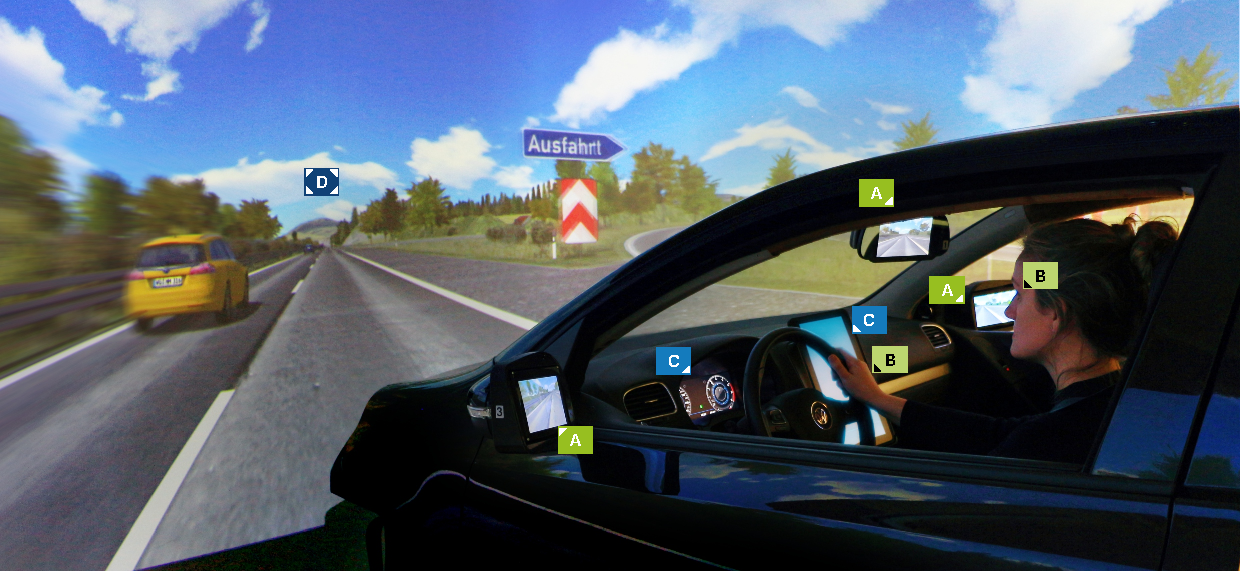
\includegraphics[width=\columnwidth]{content/caudri/images/ifab-sim1a}%
\end{nomargin} % nomargin muss vor der Caption enden, sonst ist die Caption zu breit
\caption{Der Fahrsimulator verfügt über digitale Rückspiegel (\textbf{A}) und die Möglichkeit, detailliert den Insassenzustand zu erheben (\textbf{B}), beispielsweise die Blickposition über Eye-Tracking oder Steuereingaben. Die vollständig digitalen Interieurdisplays (\textbf{C}) können nach Studienbedarf angepasst werden. Auf der 180°-Panoramaleinwand (\textbf{D}) können Fahrszenarien und Umgebungsbedingungen immersiv simuliert werden.}%
%
\end{figure*}

\newpage




Durch entsprechende frühzeitige Simulatorstudien kann sichergestellt werden, dass neue Funktionen von Anfang an menschengerecht entwickelt werden, was teuren Fehlentwicklungen vorbeugen kann. 


% Mit fquot könnt ihr ein abgesetztes Zitat aus dem Text einfügen. Ich würde es nicht zu häufig machen aber es kann Text etwas auflockern. Es ist okay, den Satz leicht anzupassen damit er besser für sich allein stehen kann.
\fquot{h}{Ein Fahrsimulator erlaubt die Erprobung verschiedenster Übergabeszenarien ohne Risiko und ohne, dass die technischen Fahrzeugfunktionen bereits real umgesetzt sein müssen.}{}

Simulatoren werden in verschiedenen Bereichen zum Training von bestimmten Fertigkeiten eingesetzt, z.B. bei der Ausbildung von Piloten mit Flugsimulatoren. Und auch im Bereich Gaming gibt es Ansätze, in denen ein Spielerlebnis mit der Vermittlung von Wissen oder Fähigkeiten verknüpft wird, sogenannte >>Serious Games<<. Die Forschung mit Fahrsimulatoren erhebt jedoch nicht den Anspruch, das Autofahren zu simulieren, sondern stelle eine >>fahrähnliche Aufgabe<< dar. Nachdem Erkenntnisse also zunächst risikofrei und kosteneffizient im Fahrsimulator erlangt werden, werden sie in der Regel im nächsten Schritt noch im Realverkehr erprobt, bevor sie im Fahrzeug umgesetzt werden.



\pagecolor{white} % Reset der (bisher schwarzen) Seitenfarbe



Der Fahrsimulator des IFAB am KIT besteht aus einem Golf-6 Fahrzeugelement, das beständig an die neuen Fahrzeuggenerationen angepasst wurde. Zuletzt wurde ein großer Mittelkonsolendisplay mit Touchfunktion verbaut, der die Bearbeitung von Nebenaufgaben oder Anzeige von Fahrzeugzustandsmeldungen erlaubt. Weitere Anzeigen, beispielsweise von Assistenzsystemen, sind im Tachodisplay möglich.

% Die Kontaktbox
\begin{wrapfigure}[20]{r}[2cm]{4cm}\vspace{-0.5cm}
\stylebox{4cm}{0.5cm}{Kontakt}{
\vspace{0.5em}
Institut für Arbeitswissenschaft \& Betriebsorganisation (IFAB)\\
am Karlsruher Institut für Technologie (KIT)

Engler-Bunte-Ring 4\\
Gebäude 40.29, Raum 006B\\
76131 Karlsruhe

Tel: +49 721-608-44250

Mail: info@ifab.kit.edu

Web: www.ifab.kit.edu\bigskip

\qrcode[height=1.5cm]{https://www.ifab.kit.edu/}
}
\end{wrapfigure}
Das Fahrzeugelement steht von einer speziellen 180°-Panoramaleinwand, auf die drei Beamer die Umgebung projizieren, die in der Software SILAB 7.1 der Firma WIVW GmbH simuliert wird. Der Blick zurück wird über Displays in den Außenspiegeln und im Innenspiegel ermöglicht. In Kombination führen die Anzeigen zu einem hohen Immersionserleben, man taucht also tief in die simulierte Umgebung ein.  Für eine möglichst detaillierte Erfassung des Fahrerverhaltens kann der Simulator mit weiteren Messsystemen kombiniert werden. Hierzu stehen dem IFAB beispielsweise Systeme zur Blickerfassung oder zur Messung physiologischer Parameter zur Verfügung.

Somit kann der Simulator am Standort Karlsruhe flexibel für eine weite Bandbreite an Studien im Bereich der Mensch-Maschine-Interaktion eingesetzt werden. Die technische Infrastruktur, sowie die Expertise zum Betrieb des Simulators und von Konzeption bis Durchführung gesamter Probandenstudien steht am IFAB für aktuelle und künftige Projekte zur Verfügung. 
\markEndOfContent % <- Das hier erzeugt die Box am Ende des Gesamtbeitrags.

\begin{figure*}[t]%
\begin{thinmargin} % Die thinmargin-Umgebung ragt in den Seitenrand-Bereich rein, aber nicht bis zur Kante. 
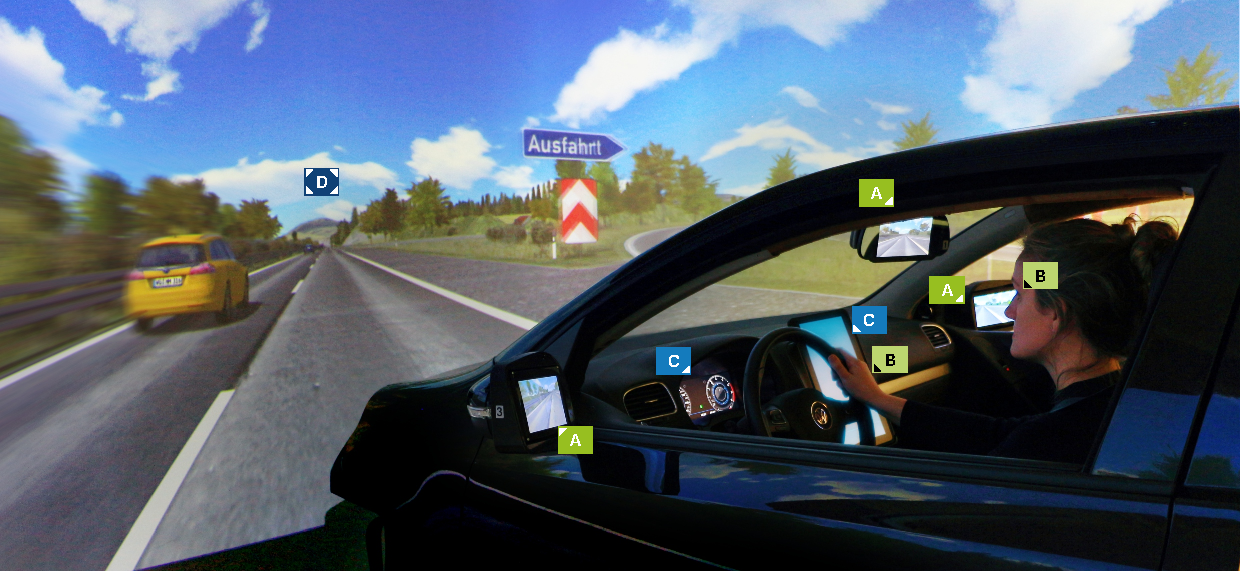
\includegraphics[width=\columnwidth]{content/caudri/images/ifab-sim1a}%

\caption{Die thinmargin-Umgebung ragt in den Seitenrand-Bereich rein, aber nicht bis zur Kante. }%
\end{thinmargin} % Bei thinmargin ist die Caption im thinmargin enthalten, sie wird also auch breiter.
\end{figure*}


\blindtext

\begin{figure*}[t]%
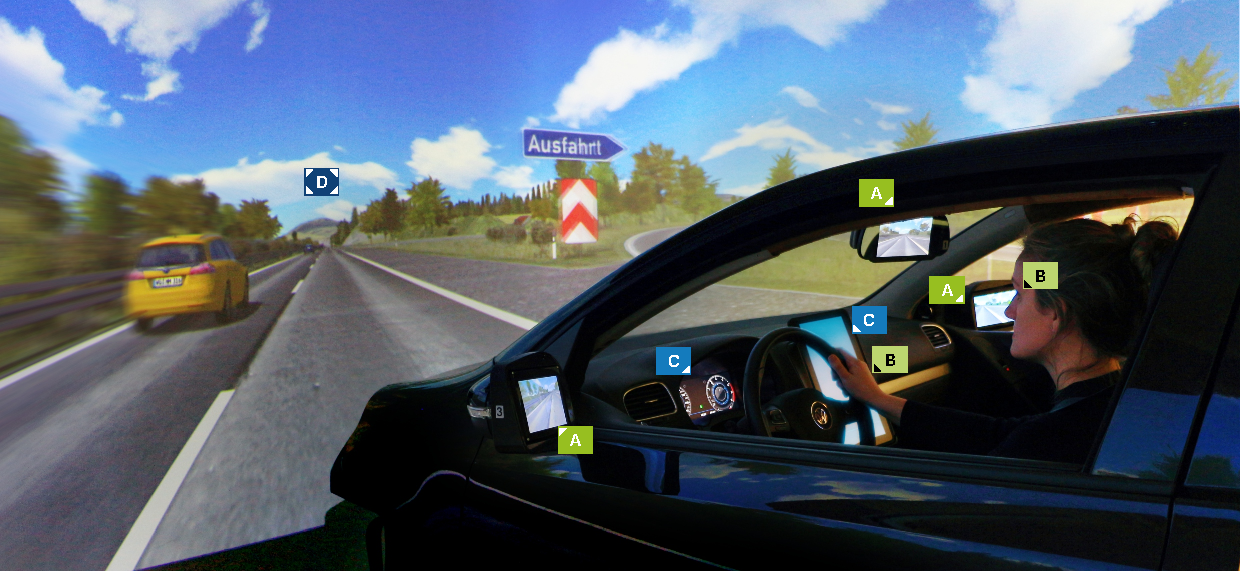
\includegraphics[width=\textwidth]{content/caudri/images/ifab-sim1a}%
\caption{Ohne thinmargin-Umgebung reichen Abbildungen nur über die Textspalten hinweg.}%
\end{figure*}



\Blindtext

% WICHTIG: Ich empfehle, als Bindestrich "= zu verwenden, wie im Beispiel unten, also Fahrzeug"=zu"=Fahrzeug"=Kommunikation zu schreiben. Dann verwendet LaTeX Silbentrennung für die Wörter "Fahrzeug" und "Kommunikation" (und "zu"). Wenn man stattdessen Fahrzeug-zu-Fahrzeug-Kommunikation schreibt, trennt LaTeX den Gesamtblock nur noch an den vorhandenen Bindestrichen, würde also das Wort "Kommunikation" bspw. nicht trennen.

\begin{figure*}[t]%
\stylebox{\textwidth}{0.5cm}{Wie funktioniert Fahrzeug"=zu"=Fahrzeug"=Kommunikation?}{

Infoboxen können den Text auch auflockern und wichtige Informationen absetzen. Sie können  \textbf{\color{colorKAMOLightBlue}einspaltig} oder \textbf{\color{colorKAMOLightGreen}zweispaltig} sein, je nachdem ob >>figure<< mit oder ohne Sternchen verwendet wird, und >>textwidth<< oder >>columnwidth<< als Breite angegeben wird.

Auch bei Infoboxen sollte man aber nicht zu viele platzieren. Ihr könnt ja mal schauen wie es bei der ersten Ausgabe aussieht.

Hier ist übrigens ein Beispiel für einen Literaturverweis \cite{ehrhardt2021gap}. Ihr müsst keine verwenden, aber wenn ihr wollt geht es so. Das Literaturverzeichnis wird >>pro Beitrag<< ausgegeben, es steht immer am Ende.
}
\end{figure*}

\Blindtext



\nocite{ziehn2023cooperative} % <- Dieser Literaturverweis erscheint nicht im Fließtext, wird aber trotzdem in das Literaturverzeichnis aufgenommen.

\printbibliography[heading=subbibliography]